
\section{Derivation of $V_{cs}$ from W leptonic branching fraction}
\label{sec:relatedWorks:vcs}


The coupling strength between \PW boson and the fermion current is $g$. However, due to the quark mixing, the vertex between  \PW boson and quark current is further scaled by a CMK element $|V_{ij}|$. Namely,
\begin{equation}
    \feynmandiagram [inline=(d.base), small, horizontal=d to b] {
        a[particle=\(\nu_e\)] -- [fermion] b [dot] -- [fermion] c[particle=\(e^-\)],
        b -- [boson] d [particle=\(W^-\)],
    };
    = i g \gamma^{\mu} , \qquad
    \feynmandiagram [inline=(d.base), small, horizontal=d to b] {
        a[particle=\(q_j\)] -- [fermion] b [dot] -- [fermion] c[particle=\(q_i\)],
        b -- [boson] d [particle=\(W^-\)],
    };
    = i g |V_{ij}|.
\end{equation}

\noindent Denoting the partial width of W decaying into one generation of lepton current $\Gamma_{W \to l \nu}$ as $\Gamma_l$, the tree-level calculation gives
\begin{equation}
    \Gamma_l \equiv \Gamma_{W \to l \nu} =  \frac{g^2 m_W}{48 \pi} .
\end{equation}


\noindent The NLO EW correction of $\Gamma_l$ is at $10^{-5}$ relatively level~\cite{dEnterria:2020cpv}, small enough to neglect. The hadronic W width decaying into $q_i,q_j$ at the leading order of QCD can be expressed in terms of  $\Gamma_l$
\begin{equation}
    \Gamma_{W \to q_i q_j}^{LO} = 3 |V_{ij}|^2 \frac{g^2 m_W}{48 \pi}  = 3 |V_{ij}|^2 \Gamma_l ,
\end{equation}


\noindent  where the factor 3 accounts for the three colors. The ratio between the total hadronic and the total leptonic W width, at the leading order of $\alpha_s$, then equals to the square sum of the CKM elements in the first two rows:
\begin{equation}
    \frac{\Gamma_{\rm had}^{LO}}{\Gamma_{\rm lep}} = \frac{\sum_{ij=(uc)(dsb)} \Gamma_{W \to q_i q_j}^{LO} }{ \sum_{e,\mu,\tau} \Gamma_l } = \sum_{ij=(uc)(dsb)} |V_{ij}|^2.
\end{equation}




% \subsection{Next-to-leading Order of $\alpha_s$}

\begin{figure}
    \centering
    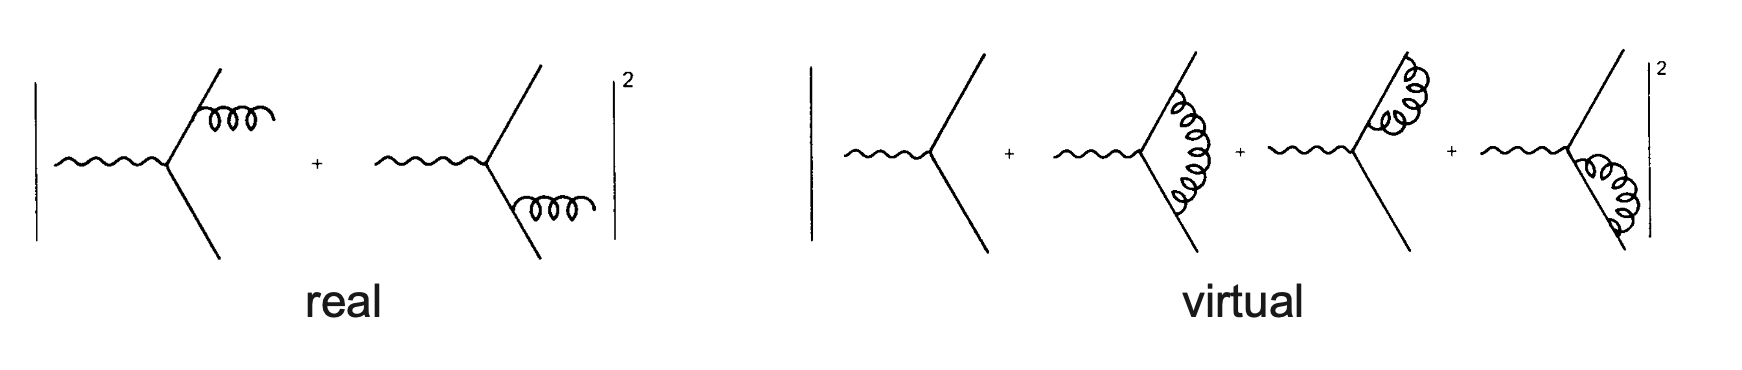
\includegraphics[width=0.8\textwidth]{chapters/RelatedWorks/sectionVcs/figures/realVirtual.png}
    \caption{ The real and virtual diagram of W decay at the NLO of $\alpha_s$. }
    \label{fig:relatedWorks:vcs:realVirtual}
\end{figure}


\noindent At the next-to-leading order (NLO) of $\alpha_s$, QCD correction related to the quark current are taken into account. More specifically, the real and virtual diagram shown in Figure~\ref{fig:relatedWorks:vcs:realVirtual} add extra contributions to the leading order width $\Gamma_{W \to q_i q_j}^{LO} $. The real diagram corresponds to the gluon final state radiation from the outcoming quarks. The virtual diagram corresponds to the interference between the tree level diagram and the virtual gluon bubbles in the quark current and at the vertex. The calculation of the real and virtual contribution is expressed as a factor multiplied on the tree level width  $\Gamma_{W \to q_i q_j}^{LO} $.
 \begin{align}
 	\Gamma^V_{W \to q_i q_j}  &= \Gamma_{W \to q_i q_j}^{LO} \times \frac{\alpha_s}{2\pi}\frac{4}{3} \bigg \{  -\ln^2\frac{m_g}{Q} -3 \ln\frac{m_g}{Q} + \frac{\pi^2}{3}-\frac{7}{2} \bigg\} \\
    \Gamma^R_{W \to q_i q_j}  &= \Gamma_{W \to q_i q_j}^{LO} \times \frac{\alpha_s}{2\pi}\frac{4}{3} \bigg \{  +\ln^2\frac{m_g}{Q} + 3 \ln\frac{m_g}{Q} - \frac{\pi^2}{3}+ 5 \bigg\}
\end{align}
 
\noindent  where $Q$ is the energy of the W boson and $m_g=0$ is the mass of the gluon, which makes both the real and virtual width diverge. But the divergences in the real and virtual width exactly cancel each other, leading to a finite total contributions. This QCD correction turns out to be a factor of $k=(1+\frac{\alpha_s}{\pi})$ :
\begin{equation}
\begin{split}
    \Gamma_{W \to q_i q_j}^{\rm NLO} =& \Gamma_{W \to q_i q_j}^{LO} + \Gamma^{V}_{W \to q_i q_j}  + \Gamma^{R}_{W \to q_i q_j}
            =   \Gamma_{W \to q_i q_j}^{LO} \big( 1+ \frac{\alpha_s(M_W)}{\pi}\big)
%             =&  \Gamma_l \bigg[ 1+ \frac{\alpha_s(M_W)}{\pi} \bigg]  \sum_{color} \sum_{ i,j } |V_{ij}|^2  \\
%             =&  \Gamma_l \bigg[ 1+ \frac{ \alpha_s(\mu_R) - \alpha^2_s(\mu_R) \frac{ \beta_0}{2\pi} \ln \frac{M_W}{\mu_R}}{\pi} \bigg] \sum_{color} \sum_{ i,j } |V_{ij}|^2  
\end{split} .
\end{equation}

\noindent Therefore at the NLO of $\alpha_s$, the ratio between the hadronic and leptonic \PW width also includes the $k=(1+\frac{\alpha_s}{\pi})$ factor:
\begin{equation}
    \frac{\Gamma_{\rm had}^{\rm NLO}}{\Gamma_{\rm lep}} =  \underbrace{(1+\frac{\alpha_s}{\pi})}_{k} \sum_{ij=(uc)(dsb)} |V_{ij}|^2.
\end{equation}


\noindent For higher order $\alpha_s$ corrections of the hadronic W width, the state-of-art factor has been calculated by considering additional QCD loops. At $\rm N^3LO$, the ratio between the hadronic and leptonic W width reads as 
\begin{equation}
    \frac{\Gamma_{\rm had}^{\rm N^3LO}}{\Gamma_{\rm lep}} =   \underbrace{ \bigg [ 1+1.045 ( \frac{\alpha_s}{\pi} ) + 0.94  ( \frac{\alpha_s}{\pi} ) ^2 -15  ( \frac{\alpha_s}{\pi} ) ^3 \bigg ]}_{k} \sum_{ij=(uc)(dsb)} |V_{ij}|^2.
\end{equation}

\noindent Finally, the sum square of the CKM elements in first two rows can be calculated by the experimental measurement of $B(W \to h)$
\begin{equation}
    \sum_{ij=(uc)(dsb)} |V_{ij}|^2 = \frac{1}{k}\times \frac{B_{W \to h} }{1- B_{W \to h}}
\end{equation}



\noindent where $\alpha_s$ at the \PW pole can be calculated with $\alpha_s(\mu_R = m_Z)=0.1178\pm0.0010$~\cite{pdg2020} and the QCD renormalization: $\alpha_s(m_W) = \alpha_s(\mu_R) - \alpha^2_s(\mu_R) \frac{ \beta_0}{2\pi} \ln \frac{m_W}{\mu_R} = 0.1199 \pm 0.0010$. The square sum of the five more precisely measured CKM elements $V_{ud},V_{us},V_{ub},V_{cd},V_{cb}$ can be calculated from the latest experimental results \cite{pdg2020} shown in Table~\ref{tab:relatedWorks:vcs:ckm}. $\rm{SS_5} = |V_{ud}|^2 + |V_{us}|^2 + |V_{ub}|^2 + |V_{cd}|^2 + |V_{cb}|^2 = 1.0490 \pm 0.0018$, which leads to the expression for $V_{cs}$:
\begin{equation}
V_{cs} = \sqrt{ \frac{1}{k}\times \frac{B_{W \to h} }{1- B_{W \to h}} - \rm{SS_5} } .
\end{equation}


% and the renormalization scale is conventionally chosen as Z mass $\mu_R=M_Z$. The running couplings derived from the higher order of QCD renormalization group equation is discussed in the Section~\ref{sec:relatedWorks:qft:qcd}. The latest PDG value of $\alpha_s(m_Z)=0.1178\pm0.0010$. Using the leading order running of coupling, the $\alpha_s$ at W pole is
% \begin{equation}
% 	\alpha_s(M_W) = 0.1199 \pm 0.0010
% \end{equation}
% By definition, the branching fraction of W satisfies the unitary constrain
% \begin{equation}
%     \sum_{ i,j } B_{W \to q_i q_j} + 3 B_l = 1
% \end{equation}

% \noindent using  $B_{W \to q_i q_j} = 3 k |V_{ij}|^2 B_l $ to substitute $B_{W \to q_i q_j}$  with $B_l$, one gets
% \begin{equation}
%     \sum_{ i,j } |V_{ij}|^2 = \frac{1}{ 3k} \, \frac{1-3B_l}{B_l}
% \end{equation}



% \noindent  With $\sum_{ i,j } |V_{ij}|^2$ and the experimental value of other 5 better measured CKM elements \cite{pdg2020} in Table~\ref{tab:relatedWorks:vcs:ckm}, we can calculate the $V_{cs}$.
